\documentclass{article}
\usepackage[utf8]{inputenc}
\usepackage{amsfonts, amsmath, amssymb, dsfont, amssymb,mathtools, multirow, tikz}



\title{Entropy}
\author{Sumit Singh}
\date{\today}

\begin{document}

\maketitle

\section{Equations}

\begin{align*}
  I(E) &= - \log[Pr(E)] = - \log(P)  \tag{Information}\\
  H(X) &= \mathbb{E}[I(X)] = \mathbb{E}[-log(P(X)] = - \sum_{i=1}^n P(x_i) \log P(x_i)  \tag{Entropy}\\
  D_{KL}(P||Q) &= \sum_{i=0}^n p(x_i) \log (p(x_i)) - \sum_{i=0}^n p(x_i) log(q(x_i)) \tag{KL Divergence}\\
  H(p,q) &= H(p) + D_{KL}(p||q) = -\sum_{i=0}^n p(x_i) log(q(x_i)) \tag{Cross Entropy}
\end{align*}

\section{Information}
\section{Gini}
\begin{equation*}
    Gini = 1 - \sum_{i=1}^n (p_i)^2
\end{equation*}
\section{Entropy}
Entropy ranges from 0 to 1, where 0 is a pure sub-tree and 1 is the most impure sub-tree. \\
Entropy for a fair sided die:\\
\begin{equation*}
    H = - \sum_{i=1}^6 \frac{1}{6} \log_2 (\frac{1}{6}) = \log_2(6) bits
\end{equation*}
\begin{tabular}{|c|c|c|}
  \hline
  \multicolumn{2}{|c|}{\textbf{Play Golf}}\\
  \hline
   $Yes$       & $No$       \\
  \hline
   $9$       & $5$       \\
  \hline 
\end{tabular}

\begin{align*}
    Entropy(Play Golf) &= Entropy(5,9) \\
    &= Entropy(0.36,0.64) \\
    &= -(0.36 \log_2 0.36) - (0.64 \log_2 0.64) \\
    &= 0.94
\end{align*}
\newpage  
\begin{figure}
  \centering
  \documentclass{standalone}
\usepackage{tikz}
\usetikzlibrary{positioning}
\newdimen\nodeDist
\nodeDist=35mm
\begin{document}

\begin{tikzpicture}[
    node/.style={%
      draw,
      rectangle,
    },
  ]

    \node [node] (A) {Root Node \{A\} 7 Yes, 5 No};
    \path (A) ++(-135:\nodeDist) node [node] (B) {\{B\} 2 Yes, 4 No};
    \path (A) ++(-45:\nodeDist) node [node] (C) {\{C\} 5 Yes, 1 No};

    \draw (A) -- (B) node [left,pos=0.25] {no}(A);
    \draw (A) -- (C) node [right,pos=0.25] {yes}(A);
\end{tikzpicture}

\end{document} 
  \caption{The enhanced diagram}
\end{figure}
\begin{align*}
    Entropy(B) &= - \frac{2}{2+4} \log_2 \frac{2}{2+4} - \frac{4}{4+2} \log_2 (\frac{4}{4+2})\\
               &= -\frac{1}{3} \log_2(\frac{1}{3}) - \frac{2}{3} \log_2(\frac{2}{3}) \\
               &= \frac{\log_2(3)}{3} + \frac{2 \log_2(1.5)}{3} \\
               &= 0.92 bits\\ 
    Entropy(C) &= - \frac{5}{6} \log_2(\frac{5}{6}) - \frac{1}{6} \log_2(\frac{1}{6}) \\
               &= \frac{5 \log_2(1.2)}{6} + \frac{\log_2(6)}{6}\\
               &= 0.65 bits
\end{align*}
    

\section{Kullback-Leibler (KL) Divergence}

\section{Cross Entropy}
\begin{center}
    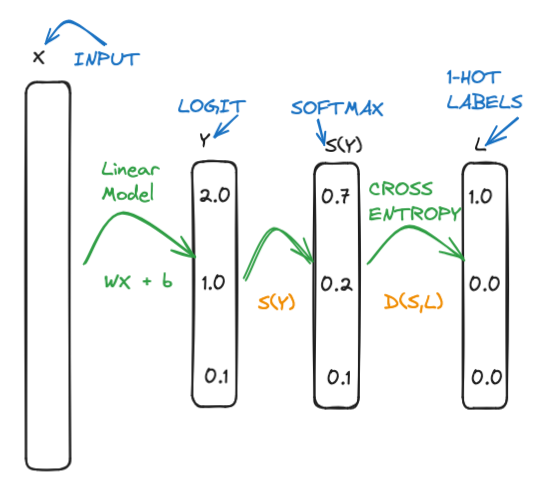
\includegraphics[width=9cm, height=6cm]{Topics/IMAGES/CrossEntropy1.png} 
\end{center}
\begin{align*}
    S(Y) &= f(s_i) &&= \frac{e^{s_i}}{\sum_j^C e^{s_j}} \\
    CE &= D(S,L) &&= - \sum_i L_i \log(S_i)
\end{align*}
\begin{itemize}
    \item In both binary and multi-class classification, cross-entropy loss calculates how close the predicted probabilities are to the true label.
    \item Lower loss value indicates better performance
\end{itemize}
\section{References}
\end{document}